\documentclass[12pt,twocolumn]{article}
\usepackage{minted}
\usepackage{amsmath,amsfonts,amssymb}
\usepackage{setspace}
\usepackage{tocloft}
\usepackage[scaled]{beramono}
\usepackage[T1]{fontenc}
\usepackage{cite}
\usepackage{authblk}
\usepackage[toc,page]{appendix} % for appendices
\usepackage{gensymb}            % for degree symbol
\usepackage[pdftex]{graphicx}   % for figures
\usepackage{siunitx}            % for si units
\usepackage[caption=false]{subfig}  % for subfigures
\usepackage{algorithm}
\usepackage{algpseudocode}
\usepackage{hyperref}
\usepackage{epstopdf}
\usepackage{titling}
\usepackage{physics}
\usepackage{esint}
\hypersetup{
    colorlinks=true,
    urlcolor=blue,
    linkcolor=blue,
    citecolor=red}
\providecommand{\keywords}[1]{\textbf{\textbf{Keywords:~}} #1}
\captionsetup[subfigure]{labelformat=brace} % setup subfigure captions
\graphicspath{{./Figures/}}     % figures in the Figures directory
\DeclareGraphicsExtensions{.eps,.ps,.pdf}    % extensions for figures
\newcommand{\comment}[1]{}      % command for multiline comments

\renewcommand{\cftdotsep}{\cftnodots}
\cftpagenumbersoff{figure}
\cftpagenumbersoff{table}
\begin{document}
\title{%
  Golfing the Method of Relaxation in Electrostatics \\
  \large and \\
    Experimental Verification That Numpy's Vector Operations are Badass}
\author{Patrick D. Cook}
\affil{Department~of~Physics,~Fort~Hays~State~University,\\Hays,~Kansas~67601,~USA}
\date{}
\begin{titlingpage}
\maketitle
\begin{abstract}
In this work, I present an overview of the method of relaxation for two-dimensional electrostatics. This method solves Laplace's equation with arbitrary boundary conditions. An implementation of the method in Python $3$ is presented with results. The problem is then "golfed" in which the shortest possible Python $3$ program which implements the method is presented, again with results.
\end{abstract}
\keywords{Electrostatics, Laplace's equation, Code Golf}
\begin{minted}[fontsize=\small]{python}
from numpy import*
from matplotlib.pyplot import*
C=30
O=10
o=10
K=roll
P=zeros((C,C))
exec('P=(K(P,1,0)+K(P,-1,0)+K(P,1,1)+K(P,-1,1))/4;P[o:-o,o:o-~O:O]=1,-1;'*9*C)
D=gradient(-P)
imshow(P)
quiver(D[1],-D[0])
show()
\end{minted}
\end{titlingpage}
\newpage
\twocolumn
\section{Basics}
\subsection{Introduction}
The equation describing the electric potential, $V$, in the absence of net electric charge is Laplace's equation\cite{Jackson99},
\begin{equation}
\grad^2V=0.
\label{eq:laplace}
\end{equation}
Carl Friedrich Gauss, of Gauss's law, proved that any function which is harmonic within some sphere---meaning that it satisfies Eq.~\ref{eq:laplace} in that sphere---has the property that its value at the center of the sphere is the arithmetic mean of its value on the surface of that sphere~\cite{Gauss}. Since the electric potential must satisfy Eq.~\ref{eq:laplace} everywhere, assuming there is no net charge anywhere,
\begin{equation}
V(\vec{r}) = \frac{1}{4\pi R^2}\oiint{Vda},~\forall\vec{r}.
\end{equation}
Where the integral is taken over the entire sphere of radius $R$ centered at $\vec{r}$. This generalizes to lower dimensions,
\begin{align}
\label{eq:3D}\mathrm{\mathbf{3D}}~&~V(\vec{r}) = \frac{1}{4\pi R^2}\oiint_\textit{Sphere}{Vda},~\forall\vec{r}\\
\label{eq:2D}\mathrm{\mathbf{2D}}~&~V(\vec{r}) = \frac{1}{2\pi R}\oint_\textit{Circle}{Vdl},~\forall \vec{r} \\
\label{eq:1D}\mathrm{\mathbf{1D}}~&~V(r) = \frac{V(r+R)+V(r-R)}{2},~\forall r.
\end{align}
This is the mathematical foundation for the method of relaxation. If the boundary conditions are known, the above equations suggest that successive averaging will converge to the solution everywhere in space. Since solutions to Eq.~\ref{eq:laplace} are necessarily unique, this will produce the only solution.

Also of importance is the electric field, which can be found from the electric potential with~\cite{Jackson99}
\begin{equation}
\vec{E}=-\vec{\grad} V
\end{equation}
\subsection{Method of Relaxation in Two Dimensions}
Suppose, instead of a continuous distribution, $V$ is instead a discrete function. Denoting $V(x_i,y_j)$ as $V_{i,j}$, Eq.~\ref{eq:2D} becomes~\cite{Jackson99}
\begin{equation}
\begin{split}
V_{i,j} = \frac{V_{i+1,j}+V_{i-1,j}+V_{i,j+1}+V_{i,j-1}}{5} \\
        + \frac{V_{i+1,j+1}+V_{i-1,j-1} +V_{i+1,j-1}+V_{i-1,j+1}}{20}.
\label{eq:2D_discrete}
\end{split}
\end{equation}
This can be seen as the weighted average of the eight neighboring points around $V_{i,j}$. The factors of $\frac{1}{5}$ and $\frac{1}{20}$ are weightings which are necessary due to the fact that the corners are farther from $V_{i,j}$ than the edges. While this equation is simple, it is only true when $V$ is the solution to Eq.~\ref{eq:laplace}. However, it can be used to find this solution. Let $V^n$ denote the $n^{\mathrm{th}}$ trial function of $V$. The initial trial function, $V^0$, will consist only of the known boundary conditions and be zero everywhere else. Given $V^n$, the next trial function is given by a modified version of Eq.~\ref{eq:2D_discrete},
\begin{equation}
\begin{split}
V^{n+1}_{i,j} = \frac{V^{n}_{i+1,j}+V^{n}_{i-1,j}+V^{n}_{i,j+1}+V^{n}_{i,j-1}}{5} \\
        + \frac{V^{n}_{i+1,j+1}+V^{n}_{i-1,j-1} +V^{n}_{i+1,j-1}+V^{n}_{i-1,j+1}}{20}.
\label{eq:2D_iterations}
\end{split}
\end{equation}
The trial functions will approach the true solution, $V$, as $n\rightarrow\infty$.
\subsection{Implementation}
Appendix~\ref{ap:fullcode} shows the implementation of the 2D method of relaxation in Python 3. The code solves for the electric potential, $V$, and electric field, $\vec{E}$, in and around a finite parallel plate capacitor.

Part of the implementation that is worth pointing out is the cyclic spacial boundary conditions. By using Numpy's \mintinline{python}{roll} function, the boundaries wrapped. For example $V_{-1,j}=V_{N,j}$ and $V_{N+1,j}=V_{0,j}$ where $N$ is the final index in the $x$ direction. This can be both advantageous and detrimental, so it is important to keep in mind.
\subsection{Results and Discussion}
Three different parallel plate capacitors were investigated using this code: one with large area and small separation distance, one with small area and small separation distance, and one with small area and large separation distance. In all cases the top plate was fixed at $-1~\si{\volt}$ while the bottom plate was fixed at $+1~\si{\volt}$. In the model, distances were not assigned to each grid point so the results are reported in arbitrary units. The results are shown below.

Figure~\ref{fig:large_A_small_d} shows the first case, large area and small separation distance. This case exhibited the characteristic strong electric field between the plates and weak electric field outside. Fringe fields are present but small.

In the second case, with small plate area and small separation distance, was very different. Figure~\ref{fig:small_A_small_d} demonstrates that the field outside the capacitor was no longer weak and that the fridge field dominated overall. There is still a stronger field inside than outside, but the magnitudes comparable.

Finally, the third case: small plate area and large separation distance. As expected, this capacitor behaves like two monopoles, as demonstrated in Fig.~\ref{fig:small_A_large_d}.

All results are qualitatively consistent with theory. Convergence testing was not performed, neither between iterations nor to analytic solutions, due to lack of interest.

\begin{figure}
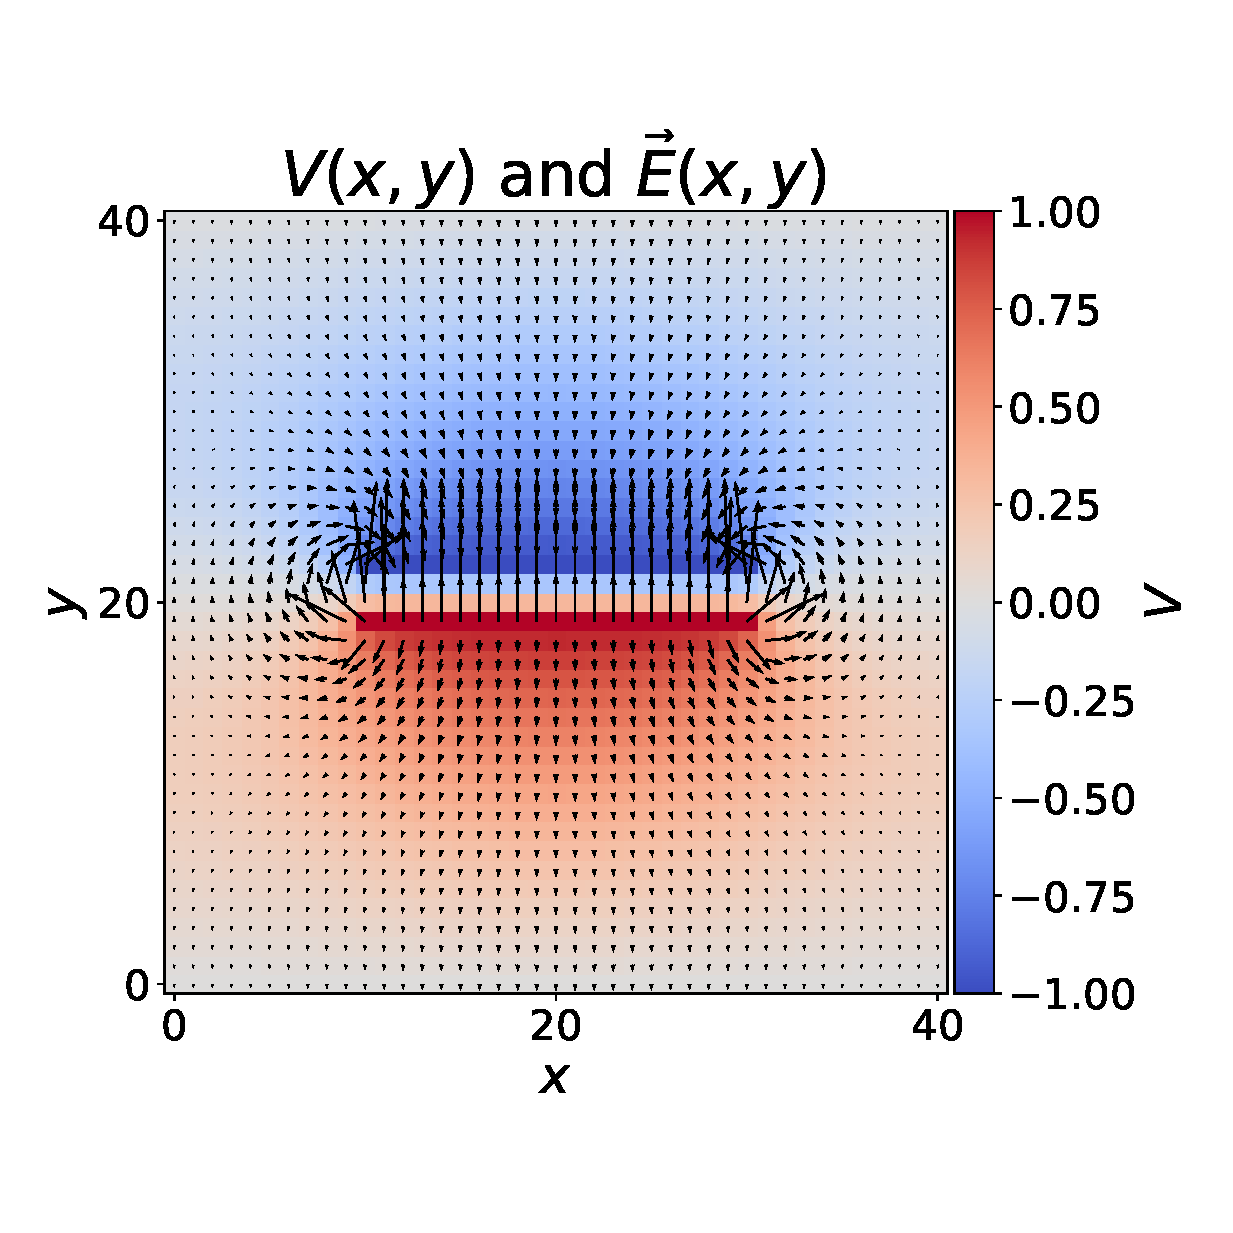
\includegraphics[width=\linewidth]{V_large_A_small_d.eps}
\caption{Capacitor with large plate area and small separation distance.}
\label{fig:large_A_small_d}
\end{figure}
\begin{figure}
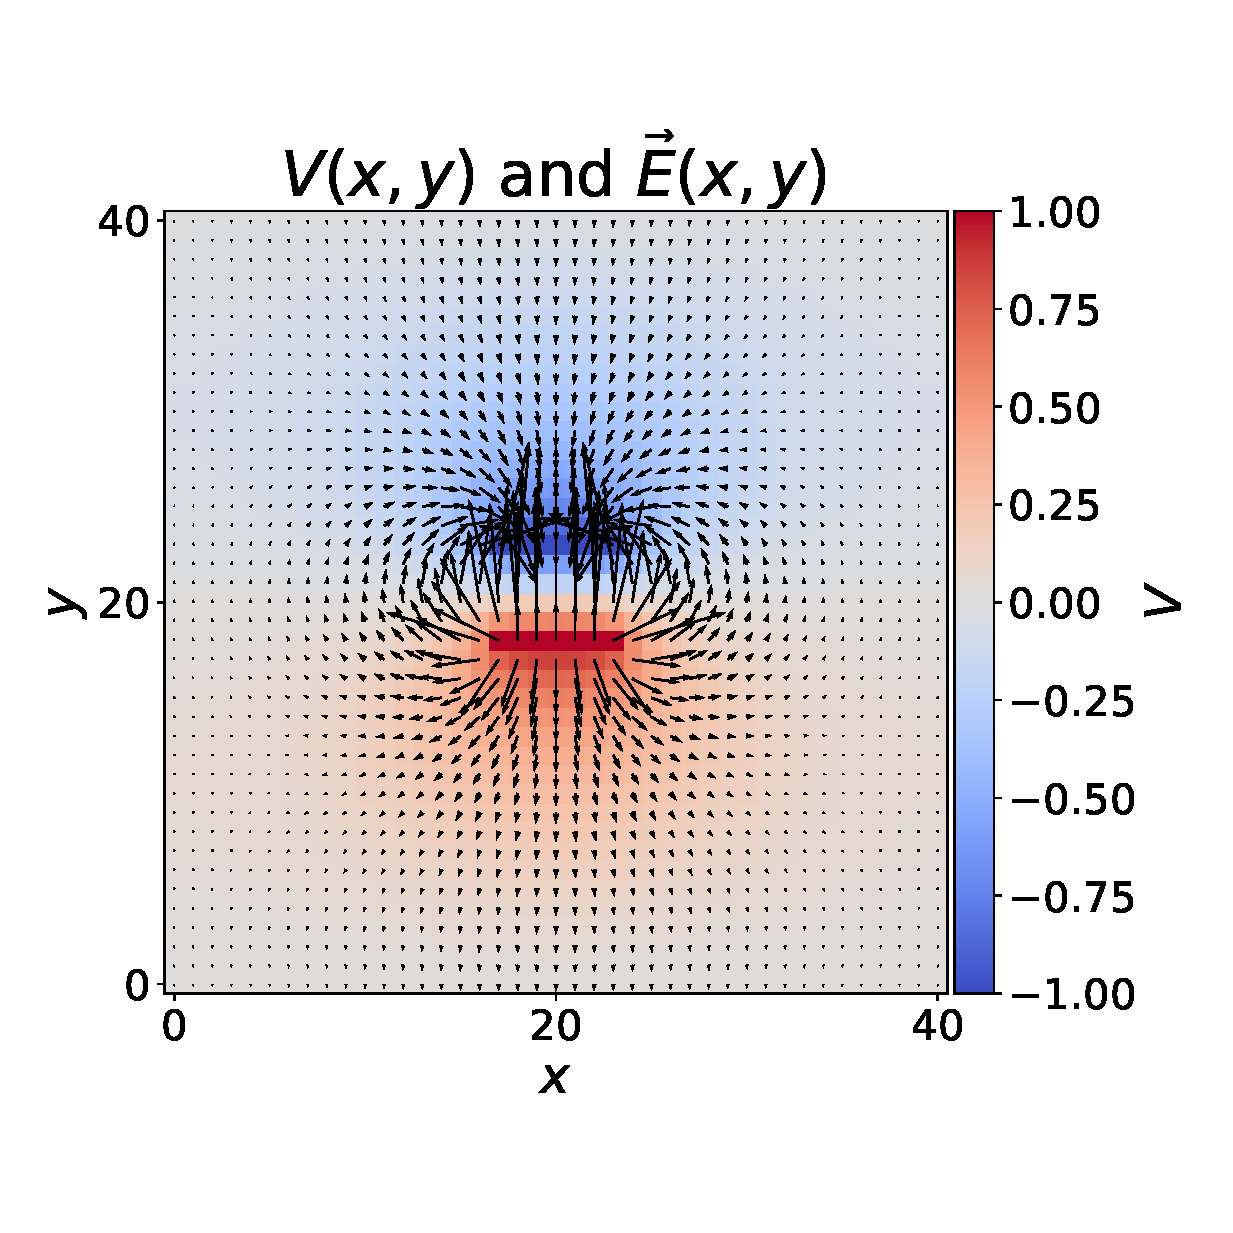
\includegraphics[width=\linewidth]{V_small_A_small_d.eps}
\caption{Capacitor with small plate area and small separation distance.}
\label{fig:small_A_small_d}
\end{figure}
\begin{figure}
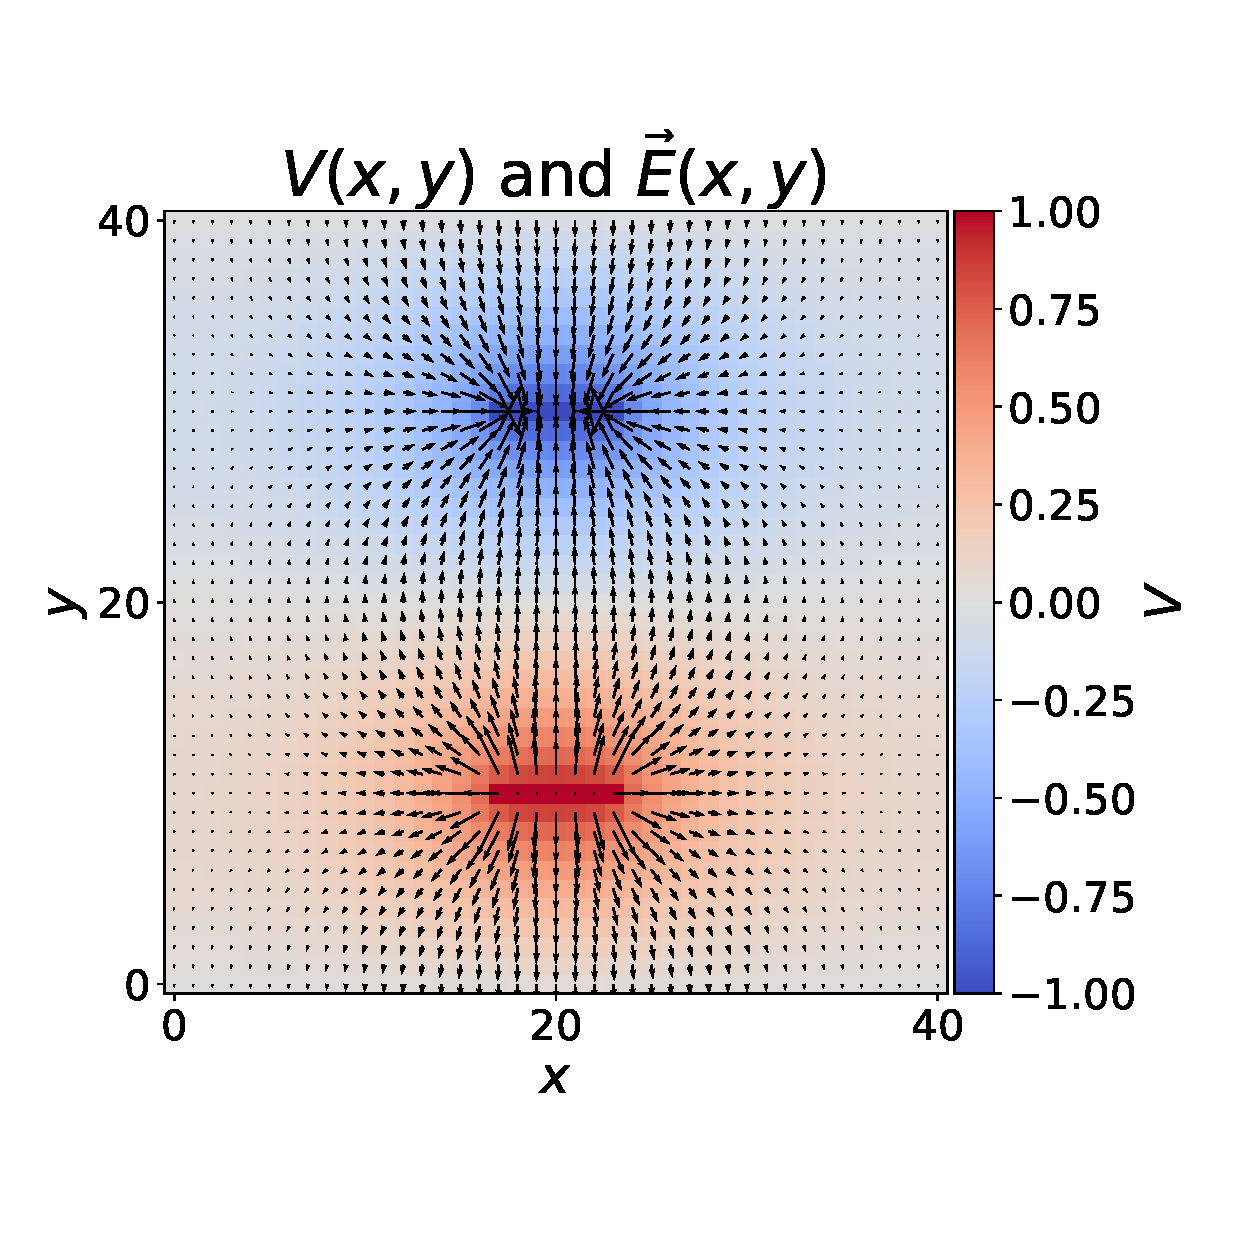
\includegraphics[width=\linewidth]{V_small_A_large_d.eps}
\caption{Capacitor with small plate area and large separation distance.}
\label{fig:small_A_large_d}
\end{figure}

\section{Code Golf}
I hope you didn't think this whole paper was going to be as boring as the last two pages. Don't worry, this isn't baby's first computational physics project. Things are about to get a whole lot more interesting. And obfuscated.
\subsection{What in the World is Code Golf?}
Code golf refers to the pastime, sport, hobby, or whatever of trying to program a task in as few characters---or bytes---as possible. There are special languages made just for this, called golf languages. These languages are often next-to-impossible to read if you're new to them. For example, here's a program that prints the first $1000$ digits of Pi, written in GolfScript:
\makeatletter
\expandafter\def\csname PYGdefault@tok@err\endcsname{\def\PYGdefault@bc##1{##1}}
\makeatother
\begin{minted}{c++}
;''
6666,-2%{2+.2/@*\/10.3??2*+}*
`1000<~\;
\end{minted}
And here's "Hello World!" in Brainfuck:
\begin{minted}[fontsize=\tiny]{c++}
+[-[<<[+[--->]-[<<<]]]>>>-]>-.---.>..>.<<<<-.<+.>>>>>.>.<<.<-.
\end{minted}
Needless to say, these aren't always useful, and should never be used in read-world applications---but they're great for golf!

Luckily, you don't need one of these fancy-schmancy languages to golf. Every language has golf potential. There are tips and tricks you could learn to golf in your favorite language, as long as it's not Java. Just please don't use those tips and tricks in real programs.
\subsection{Golfing in Python}
You could write a book on golfing in Python. Don't. In order to prepare you for the discussion to come, I will provide an overview of just a few neat golfing tricks in Python 3.

Here are some obvious golf tricks that are applicable not just in Python, but pretty much any language: remove all unnecessary spaces, use one letter variable names, don't worry about execution speed or efficiency. Okay now into the real stuff.

So starting at the top of a Python file, you'll probably have some \mintinline{python}{import} statements. Using these are kind of cheating, since you're using potentially hundreds of thousands of lines almost for free. However, I don't think anyone is going to expect you to golf a plotting engine just to plot the solution to your golfed problem, so they're alright in certain cases---unless of course the challenge was to golf a renderer. When importing Python modules, we can save a few bytes by using \mintinline{python}{from module import*} instead of \mintinline{python}{import module as m} or \mintinline{python}{from module import *}, since the space between \mintinline{python}{import} and \mintinline{python}{*} isn't necessary, and we don't want to have to type \mintinline{python}{m.} in front of every function call from that module. Of course, that means default functions may be overwritten, so you'll have to be carefull of that.

In the same realm of shortening function calls is Python's neat ability to assign new names to functions without needing to call them. For instance, say you're using \mintinline{python}{sqrt} a lot, then consider renaming the function to \mintinline{python}{s} with:
\begin{minted}{python}
s=sqrt
\end{minted}
Now, instead of \mintinline{python}{sqrt(2)}, you can write \mintinline{python}{s(2)}! This only saves bytes if you're using the function more than once. It also saves more bytes the longer the function name is.

\mintinline{python}{for} loops are messy, require indentation, and usually use \mintinline{python}{range()}, all of which take up precious bytes. If you don't care about the incremented value in the \mintinline{python}{for} loop, you can use this extremely slow, but very compact, trick:
\begin{minted}{python}
for i in range(N):
    f(x)
\end{minted}
becomes
\begin{minted}{python}
exec("f(x);"*N)
\end{minted}
Let's look at exactly what's going on here. First, lets look at the argument to \mintinline{python}{exec()}:
\begin{minted}{python}
"f(x);"*N
\end{minted}
This will evaluate to \mintinline{python}{"f(x);f(x);f(x);...;f(x)"} where there are $N$ \mintinline{python}{f(x)}'s. Now, since this is the argument to \mintinline{python}{exec()}---which runs whatever string it was given as if it were code---it runs \mintinline{python}{f(x)} $N$ times, just like a \mintinline{python}{for} loop! This saves numerous bytes in many circumstances. Of course, we can also perform standard string methods on the argument to \mintinline{python}{exec} before it runs that code, like \mintinline{python}{.replace()} or formatting with \mintinline{python}{"%s"}. These are both common tricks that are also used.

There are a few special case arithmetic operations that are important. For example, \mintinline{python}{N//M} is the same as \mintinline{python}{int(N/M)}. This means that instead of performing floating point division and converting the result to an integer, we can directly perform integer division. Also, the unary operator, \mintinline{python}{~} becomes useful to us when golfing. All \mintinline{python}{~} does is reverse the bits of the input. Nevermind what that means, but for integers \mintinline{python}{~x = -x - 1}. So we can add one and subtract one from a number by pairing \mintinline{python}{~} with \mintinline{python}{-}:
\begin{minted}{python}
-~N # same as N+1
~-N # same as N-1
\end{minted}
Now, if you're \textit{really} good at counting, you've noticed that those expressions, (\mintinline{python}{-~N} and \mintinline{python}{N+1}) have the same number of characters. So why are these useful? It's because \mintinline{python}{~} has operator precedence over \mintinline{python}{+} and \mintinline{python}{-} so instead of
\begin{minted}{python}
(N+1)/2
\end{minted}
we can save parenthesis and use
\begin{minted}{python}
-~N/2
\end{minted}

Like I said, there's a million more things to discuss about this. However, this is all we'll need for the upcoming discussion. If you're interested in learning more, just type it into Google yourself, don't come ask me.

\subsection{Numpy Arrays and Vector Operations}
Numpy is the most important thing to ever come into my life, and the same could be true for you. Learning Numpy is daunting, especially because knowing where to start is hard, but in the end it's more than worth it. I'm not saying this in terms of golfing, I mean in scientific computing, Numpy is a boon.

However, it's also great when golfing. I'm going to cover just two of the many things that make it great at golfing here, since I'll be using them in the next section.

Array indexing and slicing in Numpy is done MATLAB-style, like this:
\begin{minted}{python}
array[start:stop:step]
\end{minted}
The above code will spit out the array elements, starting at \mintinline{python}{start}, ending at \mintinline{python}{stop-1}, and skipping every \mintinline{python}{step} values. For example, suppose we have the array:
\begin{minted}{python}
array([0, 1, 2, 3, 4, 5, 6, 7])
\end{minted}
and we index it as \mintinline{python}{array[1:5:2]}, then we will get:
\begin{minted}{python}
array([1, 3])
\end{minted}
because we started at the $1^\mathrm{st}$ position, and picked every $2^\mathrm{nd}$ element, until we got to the $(5-1)^{\mathrm{th}}$ position. Importantly, this scales to higher dimensional arrays. If we have a 2D array, we can index each axis like this, separating them with commas, like \mintinline{python}{array[1:5:2,1:5:2]}.

Finally, Numpy's \mintinline{python}{roll} function is powerful. All it does is shift the positions of all the lements in an array by a specified amount, rolling elements at the end back to the beginning. It allows us to write operations which involve relative positions in arrays, like derivatives, in one line. For example, the second-order central finite difference for the second derivative is:
\begin{equation}
\frac{d^2f}{dx^2}(x_i) = f(x_{i+1})-2 f(x_{i})+f(x_{i-1})
\end{equation}
In normal Python, this would usually be implemented as:
\begin{minted}[fontsize=\small]{python}
for i in range(1,len(x)-1):
    d2f_dx2[i] = f[i-1]-2*f[i]+f[i+1]
\end{minted}
But with Numpy this can be done without the \mintinline{python}{for} loop, instead using \mintinline{python}{roll}:
\begin{minted}[fontsize=\small]{python}
d2f_dx2 = roll(f,-1) + 2*f + roll(f,1)
\end{minted}
Again, this applies in higher dimensions, it just becomes necessary to specify the axis of the roll.

\subsection{Golfing the Method of Relaxation and Its Implementation}
Here are the requirements:
\begin{itemize}
    \item The code must solve for both $V$ and $\vec{E}$ everywhere around a parallel plate capacitor using the method of relaxation
    \item The code must be able to solve any configuration of plate area and separation distance, as specified by the user (directly modifying the source is okay)
    \item Assume all user-specified numbers are two digits in base 10
    \item Both $V$ and $\vec{E}$ must be graphically displayed
    \item The number of iterations must be enough so that the results qualitatively converge

\end{itemize}

There are some tricks that can be applied to the method of relaxation itself before we start strinking our code. This is where the real golfing is done, in cleverly finagling the problem to reduce its size.

One of the easiest reductions here is that we can postpone our setting of the boundary conditions until we are done with the first iteration, since we're going to have to reset them at the end of every iteration anyways. Of course, this means the first iteration performs no useful computations, but we're not going for efficiency here.

Of course, we don't really need a rectangular domain, so I've opted for a square domain instead to save an entire line of variable assignment.

The orientation of the capacitors isn't critical, so they're vertical instead of horizontal now.

We also don't need to specify the potential on each parallel plate, since the results will scale. So we'll just hardcode them to be $+1~\si{\volt}$ and $-1~\si{\volt}$.

Again, we're not concerned with fast convergence anymore, so we can actually reduce Eq.~\ref{eq:2D_discrete} to only average the edges:
\begin{equation}
V_{i,j} = \frac{V_{i+1,j}+V_{i-1,j}+V_{i,j+1}+V_{i,j-1}}{4}.
\end{equation}
However, this feels like cheating, so I've golfed both versions, a faster-convergence method which uses Eq.~\ref{eq:2D_discrete} and a slow-convergence method which uses the above equation.

We don't want to waste bytes on making our graphs look pretty, so I've opted for whatever \mintinline{python}{matplotlib}'s defaults are.

Finally, the number of iterations can just be hardcoded to be $9N$, where $N$ is the edge length of the domain. This seems to be enough, and it doesn't require a two-digit number.

Looking at Appendix~\ref{ap:golfslow}, we see the golfed version with slow convergence. The trick of not using the corners makes the line that is iterated so short that it's not worth doing any string replacements. Therefore, it's not too hard to decode this line. Numpy's \mintinline{python}{roll} function has been renamed \mintinline{python}{r}. The line with \mintinline{python}{exec} uses the trick discussed earlier to replace a \mintinline{python}{for} loop. However, inside that line is a particularly nasty Numpy trick:
\begin{minted}{python}
V[s:-s,s:s-~d:d]=1,-1
\end{minted}
All this line is doing is setting the boundary conditions of the capacitors. But how? Well, let's look at the array indexing. The first part, \mintinline{python}{s:-s}, just says to take every element on the $y$ axis from $s$ to $-s$. The second part, \mintinline{python}{s:s-~d:d}, says to take every $d^\mathrm{th}$ element on the $x$ axis, starting at $s$ and ending at $s-~d$ (recall \mintinline{python}{s-~d=s+d+1}). If you math that out, you'll see that this will always give only $2$ elements on the $x$ axis, the element at $s$ and $s+d$. These two elements get assigned to \mintinline{python}{1,-1} corresponding to the positive and negative plates of the capacitor. That's pretty much the only cool trick in that script.

The golfed version with faster convergence, shown in Appendix~\ref{ap:golffast}, looks a lot worse, but in reality it's just a bunch of string replacement and formatting. The line where all the iterations happen, after all the replacements and formats is just:
\begin{minted}{python}
V=(r(V,1,(0))+r(V,-1,(0)) \
+r(V,1,(1))+r(V,-1,(1)))/5 \
+(r(V,1,(0,1))+r(V,-1,(0,1))+ \
r(V,1,((0,)*~-N+(1,))) \
+r(V,-1,((0,)*~-N+(1,))))/20; \
V[s:-s,s:s-~d:d]=1,-1;
\end{minted}
(Of course without all the line continuation characters,\mintinline{python}{'\'}, and linebreaks that I've added for readibility here.) Again, we see the same trick with array indexing for assigning the capacitor voltages, and the same trick with renaming \mintinline{python}{roll}. However, the last two \mintinline{python}{roll}s are worth looking at. This function call,
\begin{minted}{python}
r(V,1,((0,)*~-N+(1,)))
\end{minted}
is equivalent to an anti-diagonal roll, which in the un-golfed code was done as two consecutive rolls. All this line says is to roll $1$ over the $0^\mathrm{th}$ axis \mintinline{python}{~-N} times, then roll once over the first axis. This is the same as rolling $-1$ over the zeroth axis, then rolling $1$ over the first axis, but requires one less call to \mintinline{python}{roll}.

\subsection{Golf Results}
Figures~\ref{fig:fastgolf}~and~\ref{fig:slowgolf} show the results from both golfed codes. They're not as pretty as the un-golfed code, and they took way longer to run, but hey, the scripts are less than $300$ bytes.
\begin{figure}
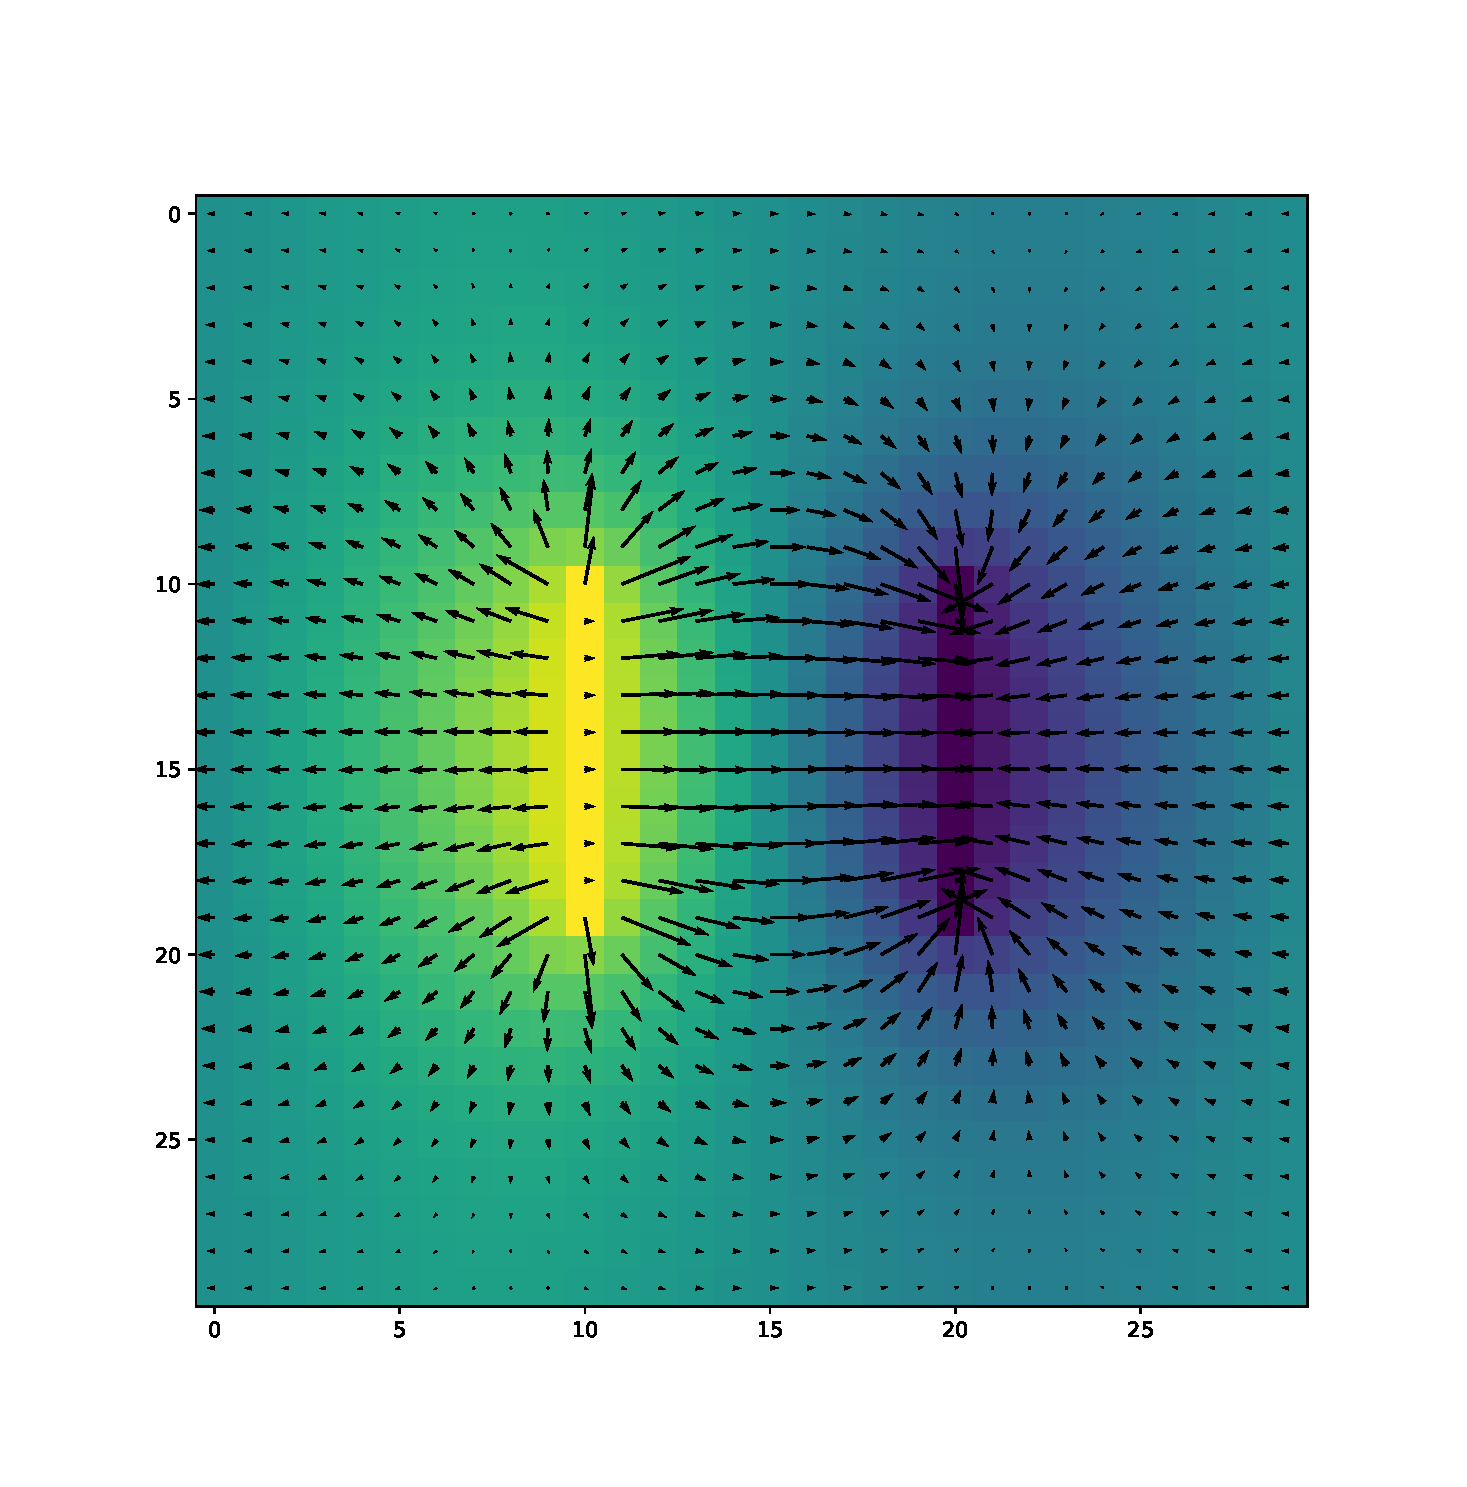
\includegraphics[width=\linewidth]{FastGolf.eps}
\caption{Output from the golfed method of relaxation using the method with faster convergence.}
\label{fig:fastgolf}
\end{figure}
\begin{figure}
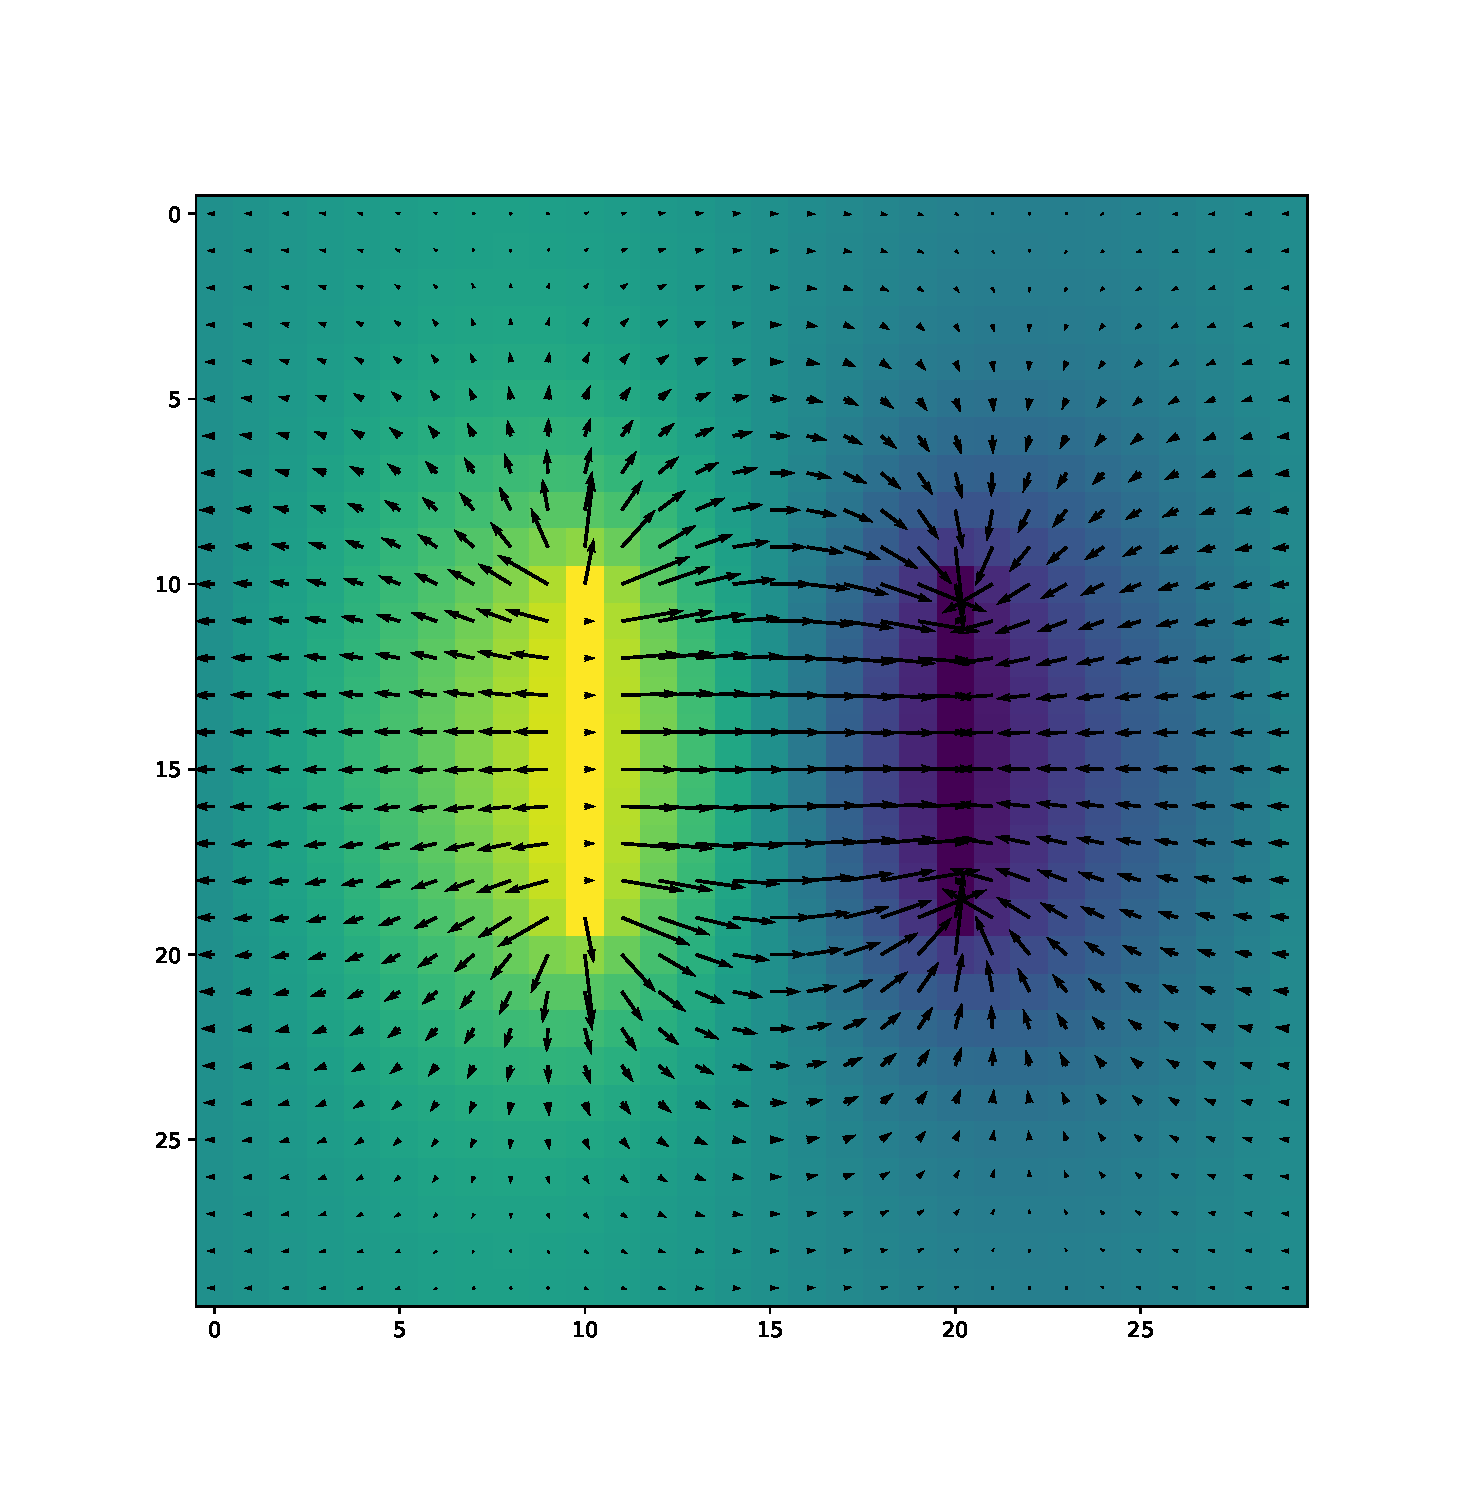
\includegraphics[width=\linewidth]{SlowGolf.eps}
\caption{Output from the golfed method of relaxation using the method with slower convergence.}
\label{fig:slowgolf}
\end{figure}

\subsection{Author's Note}
That's all I've got, hope you enjoyed. You might be wondering what's different about the code included on the title page. The answer is nothing. All I did was rename some variables so that the first column spelled out my last name and initials: Cook P. D.

\bibliography{References}
\bibliographystyle{ieeetr}
\onecolumn
\appendix
\section{2D Method of Relaxation Implemented in Python 3}
\label{ap:fullcode}
\begin{minted}[fontsize=\small]{python}
import numpy as np                                      # for arrays
import matplotlib.pyplot as plt                         # for plotting
from mpl_toolkits.axes_grid1 import make_axes_locatable # for colorbar on plots

ticks = 3 # number of ticks on x and y axis of plot

N          = 21   # size of domain in y direction
M          = 21   # size of domain in x direction
iterations = 1000 # number of relaxation iterations
distance   = 5    # gridpoints between parallel plates
width      = 5    # distance of each plate endpoint to the spacial boundary
V0         = 1    # absolute potential of each plate

# initalize the domain to zeros
V  = np.zeros((N,M))

# set the potential of both capacitors, one V0 and the other -V0
V[int(N/2-distance/2), width:M-width] = V0
V[int(N/2+distance/2), width:M-width] = -V0

# begin iterating
for _ in range(iterations):
    # Eq. 8
    V = 0.2*(np.roll(V, 1, axis = 0) + np.roll(V, -1, axis = 0) \
        + np.roll(V, 1, axis = 1) + np.roll(V, -1, axis = 1))   \
        + 0.05*(np.roll(V, 1, axis = (0,1)) + np.roll(V, -1, axis = (0,1)) \
        + np.roll(np.roll(V, 1, axis = 1), -1, axis = 0) \
        + np.roll(np.roll(V, -1,axis = 1), 1, axis = 0))

    # reset the boundary conditions (the parallel plates)
    V[int(N/2-distance/2), width:M-width] = V0
    V[int(N/2+distance/2), width:M-width] = -V0

# calculate the electric field with Eq. 6
E = -1*np.array(np.gradient(V))

# plot the results
fig,ax=plt.subplots(1,1,figsize=(8,8)) # make the figure

im = ax.imshow(V, cmap = plt.get_cmap("coolwarm"), rasterized = True) # plot V

ax.quiver(E[1],E[0]) # plot E

ax.invert_yaxis() # make the y axis point up

ax.set_xlabel("$x$",size=24) # set the x label
ax.set_ylabel("$y$",size=24) # set the y label

ax.set_xticks(np.linspace(0,M-1,ticks)) # set the x ticks
ax.set_yticks(np.linspace(0,N-1,ticks)) # set the y ticks

ax.tick_params(axis='both', which='major', labelsize=20) # change the font size

# make the axis for the colorbar
divider = make_axes_locatable(ax)
cax = divider.append_axes('right', size='5%', pad=0.05)
cbar=fig.colorbar(im, cax=cax)

# add the ticks and the label to the colorbar
cax.tick_params(labelsize=20)
cax.set_ylabel("$V$",size=24)

# set the figure title
ax.set_title("$V(x,y)$",size=30)

# save to file and show on screen
plt.tight_layout()
plt.savefig("V.eps",dpi=100)
plt.show()
\end{minted}
\newpage
\section{Golfed 2D Method of Relaxation with Faster Convergence}
\label{ap:golffast}
\begin{minted}[fontsize=\tiny]{python}
from numpy import*
from matplotlib.pyplot import*
N=30
d=10
s=10
e=exec
r=roll
V=zeros((N,N))
e("e(('V=(%s0`0`1`1)))/5+(%s0,1`0,1'+'`(0,)*~-N+(1,)'*2+')))/20').replace('`','))+%s')%(('r(V,1,(','r(V,-1,(')*4));V[s:-s,s:s-~d:d]=1,-1;"*9*N)
imshow(V)
E=gradient(-V)
quiver(E[1],-E[0])
show()
\end{minted}
\section{Golfed 2D Method of Relaxation with Slower Convergence}
\label{ap:golfslow}
\begin{minted}[fontsize=\small]{python}
from numpy import*
from matplotlib.pyplot import*
N=30
d=10
s=10
r=roll
V=zeros((N,N))
exec('V=(r(V,1,0)+r(V,-1,0)+r(V,1,1)+r(V,-1,1))/4;V[s:-s,s:s-~d:d]=1,-1;'*9*N)
E=gradient(-V)
imshow(V)
quiver(E[1],-E[0])
show()
\end{minted}
\end{document}
